%!TEX root = thesis.tex

\chapter{Robot simulation}
\label{chap:simulation}

This chapter focuses on the simulation part of the thesis. The objective is the creation of a simulation model, particularly designed for the IIS lab robot setup. The model has to reflect the properties and behaviour of the contained robot components as good as possible. Certainly the simulated components have to provide the same control interface as their real counterparts, allowing to test and optimize control code on the simulator before utilizing it on the real robot. Preferably, the control code sees no difference about on which instance it is executed. The recommendations on such a solution can be summarized as follows: 

\begin{itemize}

\item
The simulator needs to be able to generate realistic sensor and feedback data that can be used by the control software. This includes forces and torques that are measured within force sensors, the current state of the various robot joints (position, velocity, effort), but also RGB and depth images, usually produced by Kinect cameras and vision sensors.

\item
The simulation solution has to provide exactly the same ROS control interface as the real robot. This interface essentially consists of a number of ROS topics, that can be used to send control commands to the various different robot components or to read actual joint states and sensor data.
 
\item
The utilized simulation platform has to provide a graphical user interface that allows to visualize the motions of the robot and it's interaction with the environment. Possibly accidental collisions of  robot parts have to be registered and should also be visualized.

\item
In order to be used by as many people as possible, it is very important that the solution is really easy to use and does not require a long lead time. Therefore it has to be put particular focus on usability.

\end{itemize}

The following sections explain in detail, how this goal was reached. At the beginning stands the process of finding a suitable simulation platform that meets the requirements and the considered criteria. After that, the chosen simulation platform V-Rep is introduced and an overview about how to design dynamic simulations is given, explaining some of the necessary terminology. Subsequent sections focus on the necessary steps to achieve the final solution, namely finding and modelling required robot components, assembling and configuring the final simulation scene and the implementation of the ROS control interface.

\section{Choosing a suitable simulation platform}

The tasks executed on the robot are in most cases variations of so called 'pick and place' tasks. An object gets picked up, lifted and placed somewhere else within the robot's workspace. Therefore joint target positions are sent to the control interfaces of the various robot components and they execute the commanded motions if possible. The question, if the execution is possible at all and in that case in which velocity, is influenced by a number of dynamic parameters. The maximum effort of the motors in the joints is limited. If the force that acts upon a joint is higher than the maximum effort of the motor it will not be able to maintain its current position or to reach the desired target position. This can happen if the picked object is to heavy or if the robot collides with an immovable object in it's environment. The forces that act upon each single joint are influenced by a number of parameters like the position within the kinematic chain of the robot, the summed own weight of the robot components and also the weight of a possibly additional payload.

The required solution should be able to provide a realistic simulation of those dynamic interactions. Therefore the utilized simulation platform has to take use of a powerful physics engine. A physics engine is a software component, that is capable of computing parameters of physical processes and the dynamic properties of the involved objects. Examples for such engines are the Open Dynamics Engine\footnote{http://www.ode.org} (ODE) and Bullet physics\footnote{http://bulletphysics.org}. Some of the evaluated simulation platforms even provide a number of different physics engines to choose.\\

The candidates that have been taken into account were Gazebo\footnote{http://gazebosim.org/}, V-Rep\footnote{http://coppeliarobotics.com}, MORSE\footnote{http://www.openrobots.org/wiki/morse/} and Openrave\footnote{http://openrave.org}. After some investigation only two of them (Gazebo and V-Rep) had been evaluated in greater detail. Criteria for the selection had been:

\begin{itemize}
\item
Which physics engine is used respectively is it possible to choose among various engines?
\item
Usability and stability
\item
Expandability
\item
Availability of required model components (arm model, gripper,...)
\item
Quality of the documentation
\item
Licence issues
\end{itemize}

Taking into account those criteria it went clear that V-Rep will be the simulation platform of choice. In some initial tests V-Rep seemed to be much more stable than Gazebo and the user interface is very intuitive. Another important point is that V-Rep ships with a fully functional model of the KUKA LWR4+ robot arm.

\section{The Virtual Robot Experimentation Platform(V-Rep)}
V-Rep is a powerful robot simulation platform, developed by Coppelia Robotics. The current version (V3.1.2) provides the ability to choose from three configurable physics engines (ODE, Bullet, Vortex -- only trial version) for simulating dynamic processes. It also contains a very comfortable editor for modelling robot components and simulation scenes. In the \emph{shape edit mode} it is possible to edit and simplify meshes. This is very important because for simulating dynamic processes only simple shapes with a low amount of vertices, edges and faces should be used to reduce complexity. The contained model browser provides a rich set of different robot models, static objects and various sensors, ready to use. A powerful feature are V-Rep's so called \emph{calculation modules}. They can be configured to provide additional calculation functionalities on groups of scene objects. The \emph{collision detection module} is capable of detecting and visualizing all kinds of collisions within the simulation scene. The \emph{inverse kinematics calculation module} allows to solve inverse kinematics problems for robot components. The behaviour of the simulator is highly customizable via a rich programming API for C++ as well as the scripting language LUA\footnote{http://www.lua.org}. V-Rep is no open source software but it provides a free licence for educational units and can therefore be used for research purposes. A more detailed introduction to V-Rep can be found in \cite{freese2013}.

\section{Dynamic simulations in V-REP}
For a better understanding of the modelling process it is necessary to explain a few fundamental concepts about designing dynamic simulations in V-Rep. This section just covers those aspects that are important for the underlying project. A more detailed explanation can be found in the official V-Rep documentation\footnote{http://www.coppeliarobotics/helpFiles}. \\

Each simulation scene in V-Rep is composed from a number of models that are arranged within the environment. A model consists of various scene object, combined in a tree like structure to mimic the kinematic chain of a robot component. Each model has a dedicated model base and constitutes a sub-tree of the scene hierarchy. The model base is the root element of the model tree. There are existing various types of scene objects within V-Rep, but only those, which are important for the implementation will be explained here.

\begin{itemize}
\item \textbf{Shape} \\
A shape is a 3 dimensional body. Shapes represent the visual parts as well as the dynamically enabled parts of the scene. It is necessary to distinguish between primitive shapes (Cylinder, Cuboid, Sphere, Plane and Disk) and complex shapes (triangle meshes). Primitive shapes are much easier to handle for the physics engine as there can happen a lot of optimization during dynamics calculations. Complex shapes usually look better and therefore they are used mainly as the visual part of the model but also by the collision detection module. Various shapes can be combined to groups and therefore treated as one single object. Shapes can be defined as \emph{static} or \emph{non-static} objects. The position of a static object is fixed relative to it's parent node within the scene hierarchy and will not change during simulation. Non-static objects underlie gravity and will fall down if they are not constrained by a dynamically enabled joint or a force sensor connection. It is also necessary to distinguish between \emph{respondable} and \emph{non-respondable} shapes. Respondable shapes have a clearly defined mass and moment of inertia and therefore they create collision reactions when colliding with other respondable objects during simulation. Only respondable shapes are considered during dynamics calculation. Usually a model in V-Rep is composed of a visual part, consisting of complex shapes and a hidden part, consisting of groups of primitive shapes that are configured to be used for the dynamics calculations. This issue will be covered again when explaining the creation of the hand model. Each shape also has some additional flags, defining special attributes used by the \emph{calculation modules}. The \emph{collidable} attribute states that a shape has to be considered during collision detection. The \emph{renderable} flag marks a shape to be recognized by a \emph{vision sensor}. There are more flags available but only those two were used within this project.

\item \textbf{Joint} \\
A joint is a flexible connection between two rigid parts of a robot. It has to be distinguished between revolute or prismatic joints with one degree of freedom and spherical joints with three degrees of freedom. In the arm and hand model only revolute joints are used. Joints can be passive or actuated by a motor. The motor settings include maximum force or torque and velocity limits. If the control loop is enabled then a desired target position for the joint can be set. The controller will then try to reach this position, based on it's PID settings while respecting the motor limits. It would also be possible to program a custom control loop for each joint but for the current project this is not necessary. Joints can be operated in various different modes. A joint in \emph{torque/force mode} is simulated, using the physics engine. This is the most realistic control mode. A joint in \emph{inverse kinematics mode} is controlled by the inverse kinematics calculation module and if additionally the option \emph{hybrid operation} is selected then the dynamic parameters of the joint are also taken into account. Operating a joint in \emph{dependent mode} means that it's position depends on the position of another joint within the scene. How this dependency looks like can be configured by setting a \emph{dependency equation}.

\item \textbf{Vision sensor} \\
States a simulated image capturing device. A vision sensor can capture images of the simulation scene, depending on it's configuration. It can deliver RGB image sequences as well as depth images. Vision sensors are used in the Kinect camera model.

\item \textbf{Force sensor} \\
A force sensor in V-Rep is a rigid connection between two dynamically simulated objects. The calculated forces and torques can be measured and visualized. It is also possible to define a maximum force the connection is able to bear. When this maximum value is exceeded, the connection will break.

\item \textbf{Dummy} \\
Dummies are the simplest scene objects at all but they provide some important functionality, especially for the various calculation modules of V-Rep. They can be understood as the origin of a named reference frame with a configurable position and orientation within the simulation scene. Two dummies can be linked as \emph{tip-target pairs} to be used by the IK calculation module. The importance becomes more clear when the construction of the simulation scene will be explained, particularly when configuring the inverse kinematics calculation module. 

\end{itemize}

Groups of scene objects can be organized in collections and treated as one single entity. Collections play an important role in the collision detection module.


\section{Designing the simulation scene}
This section explains in detail the structure of the simulation scene and the contained model components. The setup contains three types of robot component - the Kuka LWR4+ robot arm, the Schunk SDH-2 gripper and the Kinect camera. For each one of them, a simulation model was required in order to be able to build up the scene. V-Rep ships with realistic and fully functional model for the Kuka arm and also for the Kinect camera. But as there is currently no model for the Schunk gripper available, it had to be created from scratch. The necessary steps of the modelling process are explained in the next section.

\subsection{Modelling the Schunk SDH-2 gripper}

A model within a V-Rep simulation scene basically consists of three major parts. First there are the shapes that form the visual part of the model. Those shapes are triangle meshes for each single link of the robot component. Preferably they are not to complex, i.e. the amount of faces is not to high. The second part is formed by the joints that connect those shapes and allow to actuate the flexible parts of the model. The third part consists of the dynamically enabled parts of the model. Theese shapes form the body of the model, how it is seen by the physics engine. Those respondable parts are usually an approximation of the original meshes, composed from groups of primitive shapes. Those parts are very important as they make the model realistic and allow to interact with other respondable objects within the scene. Without them, the model would just move through other bodies as only respondable shapes are able to produce collision reactions. The steps, described within this section enclose the modelling of that three parts for the gripper model.\\

\begin{figure}[ht]
	\centering
  	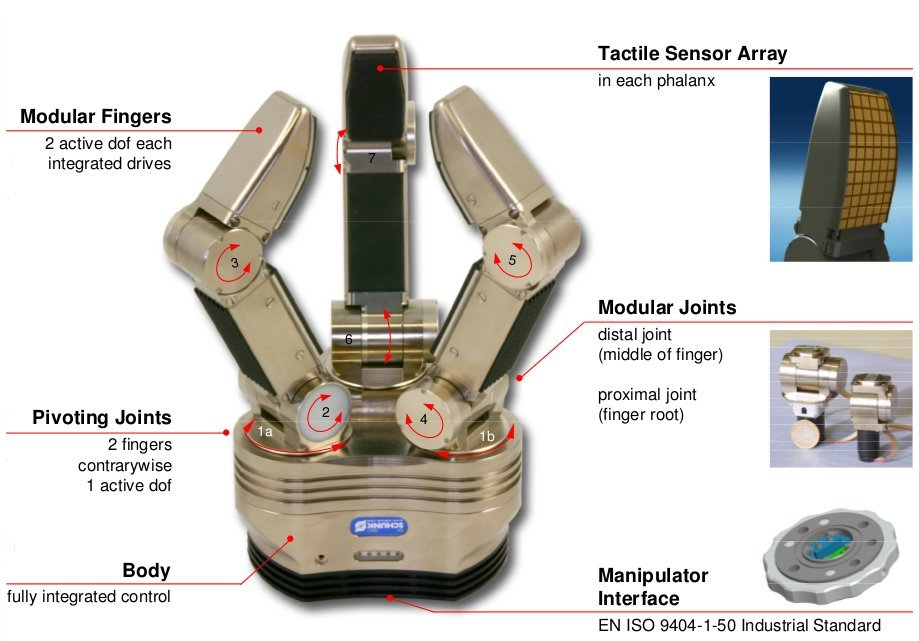
\includegraphics[width=1.0\textwidth]{images/sdh_sheet.jpg}
	\caption{Schunk SDH-2 gripper}
	\label{fig:sdh_sheet}
\end{figure}

Figure\ref{fig:sdh_sheet} shows the Schunk SDH-2 hand. The gripper has 3 fingers, each one containing two modular joints. The joints located closer to the wrist are called the \emph{proximal} finger joints whereas the joints, actuating the finger tips are called the \emph{distal} finger joints. Two of the fingers can be rotated along their vertical axis but they are connected contrariwise. That means if one finger rotates to the left, the other one is rotated to the right for the same angle, actually adding one additional degree of freedom. Those two joints are called the \emph{pivoting} joints. The visual part of the hand model basically consists of 4 different shapes - the wrist, finger knuckles, finger links and finger tips. Suitable meshes were taken from the schunk\_description\footnote{http://wiki.ros.org/schunk\_description} ROS package and imported into the V-Rep robot editor. They have then been arranged according to the technical description. The next step was to insert and arrange the gripper joints on their appropriate locations.

\begin{figure}[t]
	\centering
  	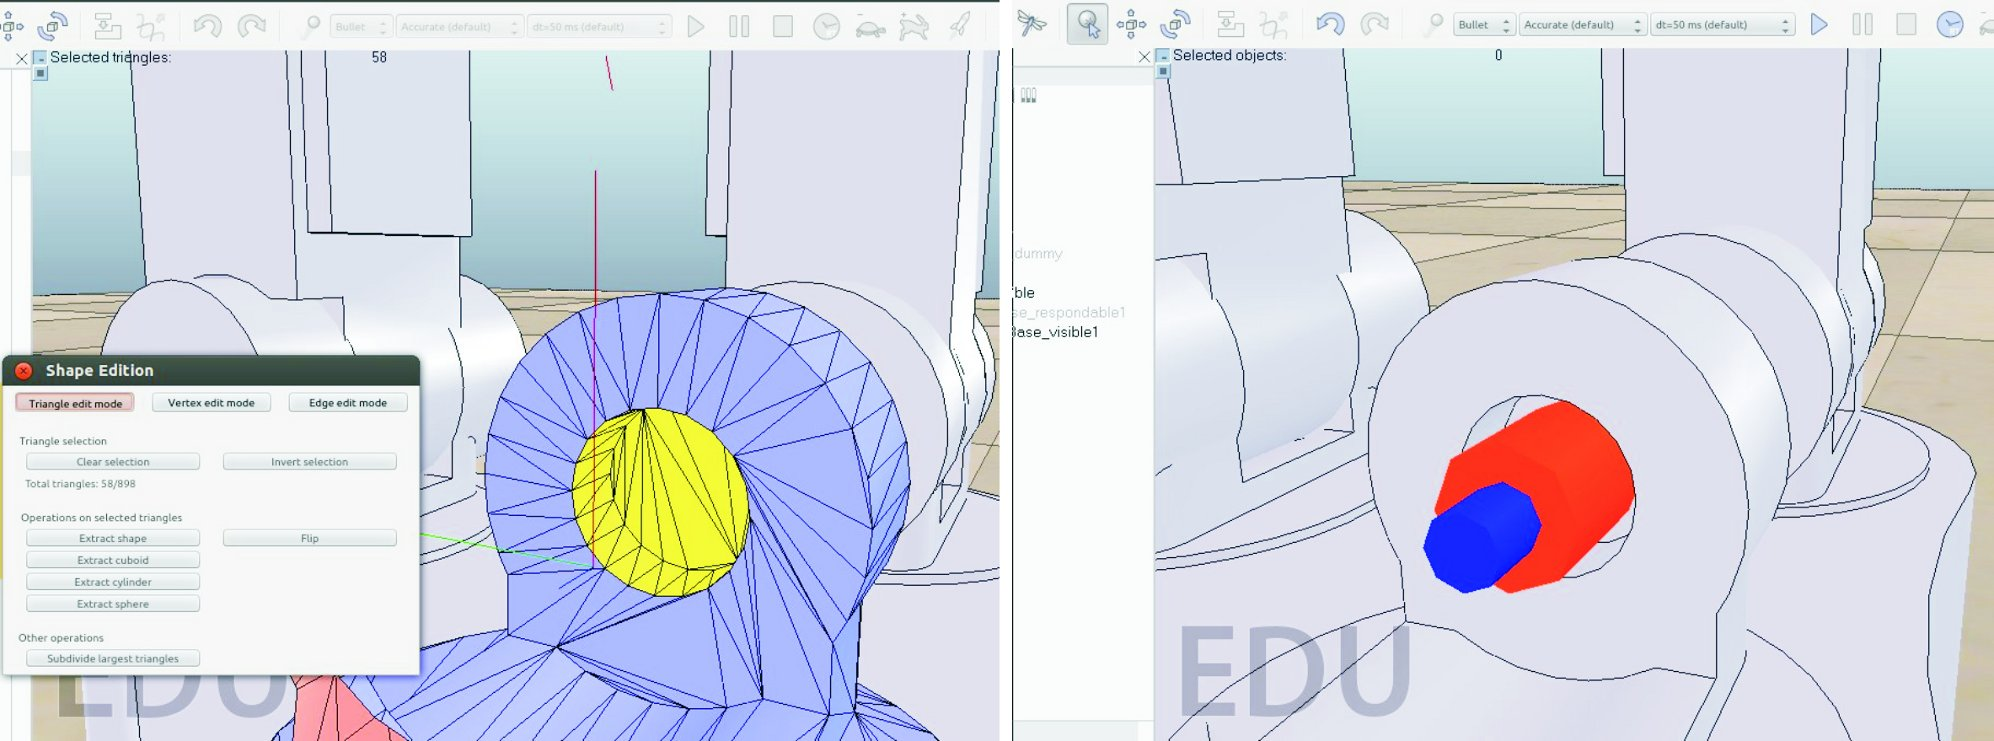
\includegraphics[width=1.0\textwidth]{images/place_joint.jpg}
	\caption{Placing a joint within the model}
	\label{fig:place_jnt}
\end{figure}

Therefore it was important to determine the correct position and orientation for each single joint within the model to allow the correct movement of the fingers. This was achieved by using the \emph{shape edit mode} and select the cylinder shaped area within the mesh, where the joint has to fit. From that selection a cylinder was extracted and the joint was then centred within this newly created cylinder. Those steps had to be repeated for all 8 joints. The placement process can be seen in Figure\ref{fig:place_jnt}.

\begin{figure}[b]
	\centering
  	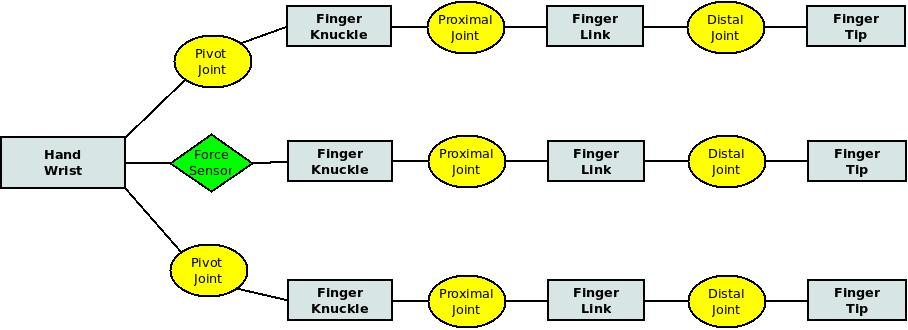
\includegraphics[width=1.0\textwidth]{images/hand_tree.jpg}
	\caption{Kinematic chain of the Schunk gripper}
	\label{fig:hand_tree}
\end{figure}

The left image shows the extraction on the target area. On the right image, the joint is already placed on it's appropriate location.\\

After placing all the joints and links within the scene, the model tree was adjusted to form the kinematic chain of the hand as can be seen in Figure\ref{fig:hand_tree}. The dynamic parameters of the joints were set according to the technical description. Those parameters include the joint limits, maximum velocity and maximum effort. As the positions of the pivot joints are connected to each other, the configuration of the second finger's root joint looks sightly different. To achieve this mirroring behaviour the joint is operated in the \emph{dependent mode}, which means it's position \emph{depends} on the position of a connected joint and that dependency is expressed as \emph{dependency equation}. The configured equation just copies the actual position but the joint is operated in opposite rotational direction.\\

The meshes only form the visual part of the model, but they are to complex to be used for dynamics calculations. So the shape of each link had to be approximated by groups of primitive shapes. This was achieved by executing the following steps for each single part of the model:
\begin{itemize}
\item
Within shape edit mode locate parts of the mesh that could be approximated by a primitive shape (cuboid, cylinder), by selecting suitable groups of vertices
\item
Extract the primitive shape by using the corresponding editor functionality
\item
Repeat those steps until the most important parts of the link are approximated that way
\item
Group those primitive shapes to treat them as one single object
\item
Adjust the dynamic parameters (mass, material settings, inertial matrix)
\item
Adjust the local respondable mask
\item
Give the group the same name as the corresponding mesh, but with the \emph{\_res} suffix
\item
Remove the extracted shapes from the current visibility layer because they are just used for dynamics calculations
\end{itemize}
\begin{figure}[ht]
	\centering
  	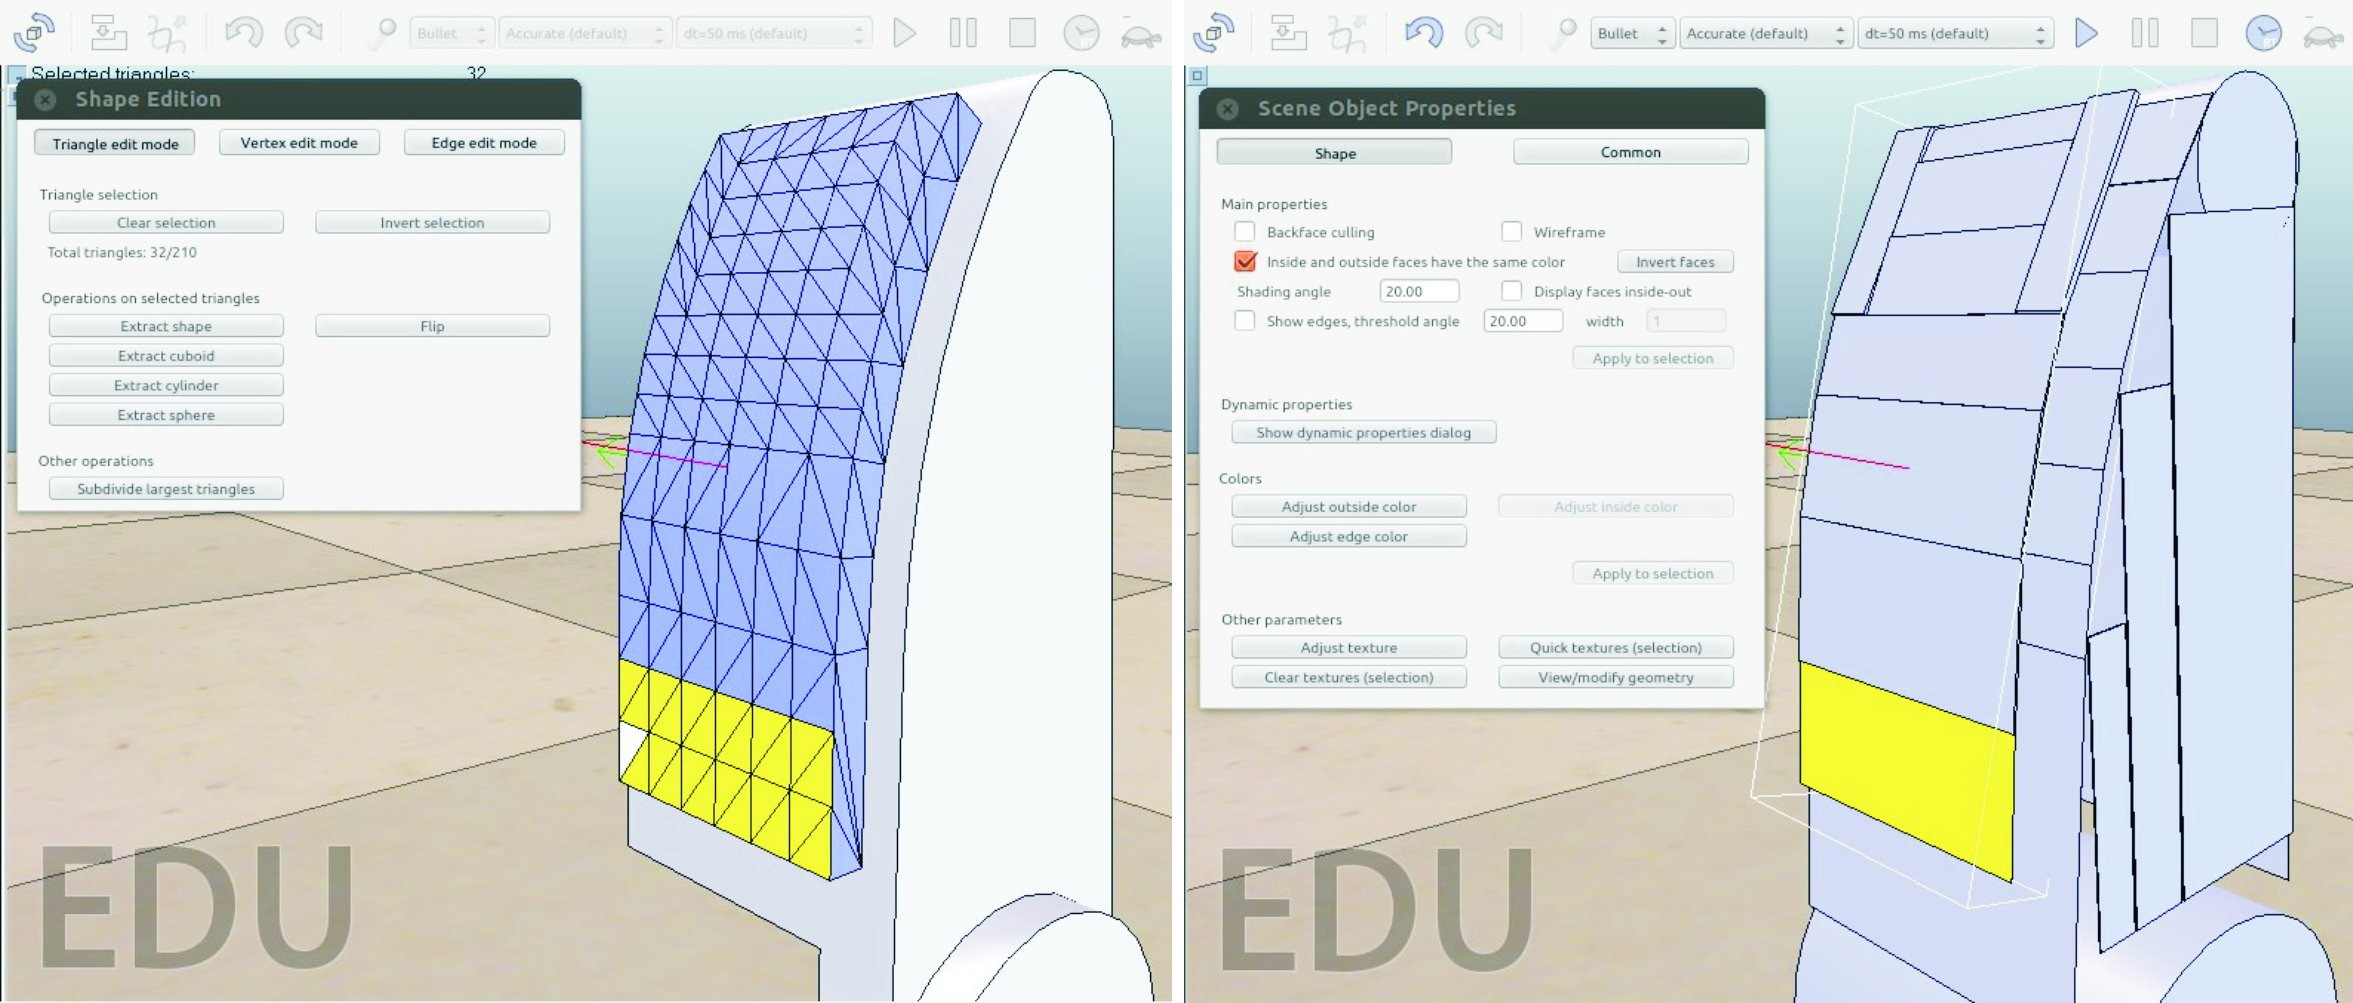
\includegraphics[width=1.0\textwidth]{images/extract_pure_shapes.jpg}
	\caption{Process of approximating the original mesh with pure shapes}
	\label{fig:ex_pure_shape}
\end{figure}
The extraction process is visualized in Figure\ref{fig:ex_pure_shape}. Dynamic parameters like mass and inertial matrix have been provided by Alex Rietzler. The predefined \emph{highFrictionMaterial} setting was used for each single part of the finger because that showed better results when picking up objects later on.\\

The last step of the modelling process was the adjustment of the model hierarchy. Root element of the hand model is the respondable part of the wrist which is also the dedicated model base. It is very important to follow the V-Rep guidelines for designing dynamic simulations because if the hierarchy is wrong, the model will simply fall apart when starting the simulation (detailed information can be found in the corresponding chapter\footnote{http://www.coppeliarobotics.com/helpFiles/en/designingDynamicSimulations.htm} of the V-Rep dodumentation). Each non-static and respondable shape has to be connected to it's parent by a joint or a force sensor. The visual part of the link is always a child object of it's corresponding respondable. That way, the kinematic chain of the gripper is formed.


\subsection{Assembling the scene}

\begin{figure}[ht]
	\centering
  	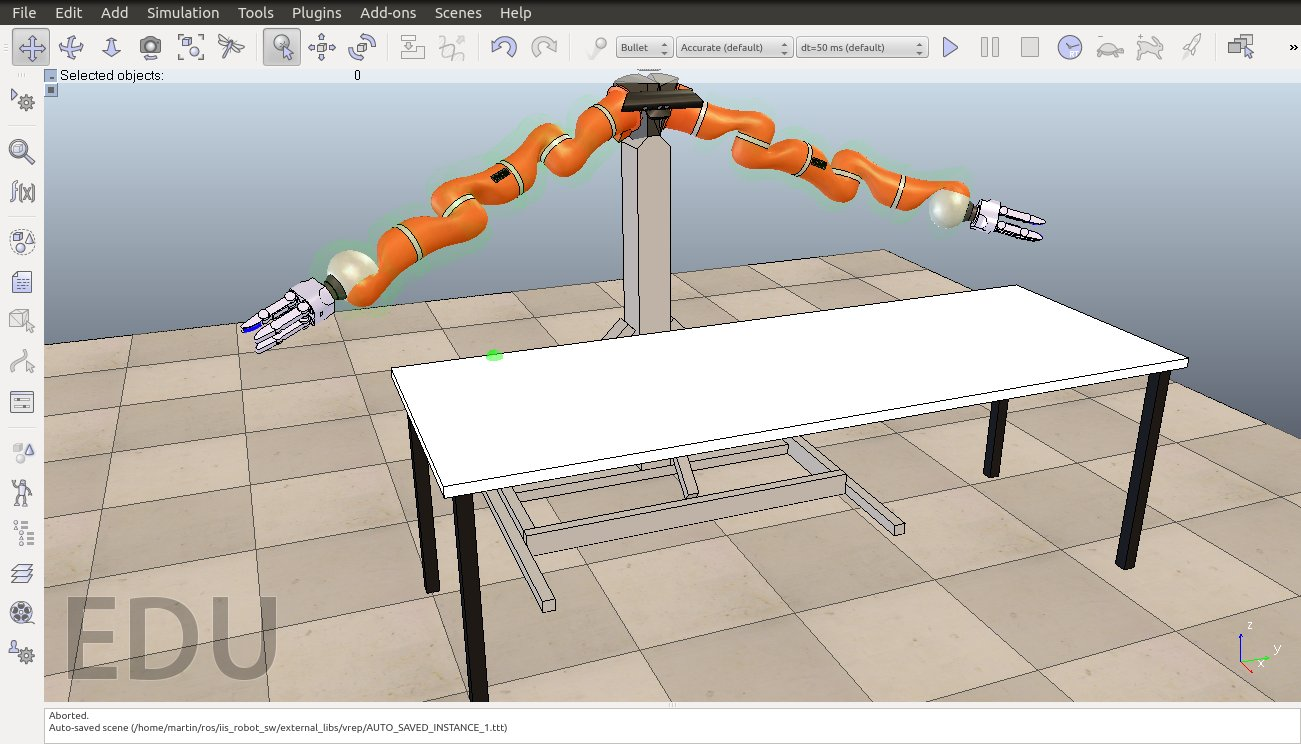
\includegraphics[width=1.0\textwidth]{images/simulation_scene.jpg}
	\caption{Structure of the V-Rep simulation scene}
	\label{fig:sim_scene}
\end{figure}

After finishing the gripper modelling process, each necessary component was available to build up the simulation scene as can be seen in Figure\ref{fig:sim_scene}. The final scene consists of a model of the robot's torso, two KUKA LWR4+ arm models with attached grippers and a model of the table in front of the robot. The origin of the world reference frame is located on the upper left side of the table, indicated by a slightly green shimmering sphere. A dummy object called \emph{ref\_frame\_origin} was placed at that location. Each position calculation later on will happen relative to that dummy element. If it is necessary to move the origin to another location within the workspace, this can simply be achieved by just moving that dummy to the required location. The position and orientation of the torso, the table and the two arms are set relative to the world reference frame. (TODO: transformation was provided - how was it achieved?). The grippers were placed on the tip of each arm. Within the scene hierarchy they are child elements of the last node in the corresponding arm tree. The correct rotation and offset was measured on the real counterpart and then adjusted accordingly. \\

The plate and the legs of the table were modelled as group of primitive cuboids. The table is defined as respondable to ensure that it will produce a collision reaction if a robot component collides with it. But as it is a static object it's position will not be influenced by such a collision because it is fixed within the scene. The material setting is set to \emph{highFrictionMaterial}. \\

The Kinect camera model was also taken from the model browser. As it's position and orientation in the real world is not fixed and might change from time to time, it's position within the simulation scene is just an approximation to reflect the real world setting as good as possible. 

\subsection{Configuring the collision detection module\footnote{http://www.coppeliarobotics.com/helpFiles/en/collisionDetection.htm}}

One of the requirements to the final solution is the ability to detect and visualize possible accidental collisions of the simulated robot with itself or it's environment. Moreover it would be a convenient feature to have some kind of warning if some of the robot's parts come dangerously close to an obstacle during movement. This could be achieved by using a padded version of the robot model for additional collision checking.
 

 These considerations led to two different types of possible collisions. \emph{Soft collisions} are collisions, detected using an enlarged version of the robot model. They just indicate a warning that the robot comes very close to an object it is not allowed to collide with. \emph{Hard collisions} mean that a robot component directly hits another collidable object. This would be also a collision in the real world. The simulator should be able to distinguish cleanly between those two types of collisions.\\ 

The goal was achieved by using V-Rep's \emph{collision detection module}. This calculation module can be used to detect and visualize all kinds of collisions within the simulation scene. The first necessary step of the configuration process was to create the \emph{collision shield} - a collection, consisting of enlarged copies of the robot links. Therefore it was necessary to model an additional shape for each link that is slightly larger than the original one. This modelling process started at the second link of each robot arm and on all subsequent links the following steps had to be performed:

\begin{itemize}

\item
Create a copy of the shape that forms the visible part of the robot link
\item
Morph the copied object into a group of convex shapes to reduce complexity. This can be done by using the corresponding shape editor functionality.
\item
Ungroup the resulting group of shapes and merge them into one single shape
\item
Grow the resulting shape, but only in x and y direction of it's own reference frame. The resulting mesh should be approximately 10cm larger while still having the same height.
\item
Adjust the outside color to make it green and nearly transparent. The collision shield should be visible but not completely occlude the original model.
\item
Rename the shape to the same name as the original one but add the '\_col' suffix to be be able to easily identify it within the model hierarchy.
\item
Make the new shape a sibling of the original one within the model tree
\item
Adjust the shape object properties. Define the new shape to be \emph{static} and \emph{non-respondable}.
\item
Disable the \emph{collidable} flag on the shape. This behaviour will be overridden in the collection
settings later on when configuring the collision detection module.

\end{itemize}

This modelling process is visualized in Fig???.\\

The next step was to adjust the configuration of the \emph{collision detection module}.

. Therefore a number of so called collision objects have to be configured within V-Rep's collision detection module. Each collision objects checks for collisions between a collider against a collidee. Collider and collidee are single shapes or collections of shapes with the collidable flag set. For each arm two collision objects have to be set up - one for each collision type. The configuration is explained for the left arm but the steps for the right arm are similar. The first collision object is named 'left\_arm'. The collider is the collection called 'leftArm'. This collection contains the whole sub tree of the left arm, including the gripper, but excluding the elements of the left collision shield. The collidee are all other collidable entities within the scene. This collision object detects the hard collisions. This also makes clear, why the collidable flag is disabled on the parts of the collision shield because otherwise collisions with the shield would also be detected which would not be correct. The second collision object is called `left\_armShield'. The collider is the collection called `leftArmShield'. This collection is composed of the parts of the left collision shield and the whole subtree of the left gripper. This collection is defined to override the value of the collidable flag of the contained elements - this is important because as previously mentioned, the elements of the collision shield are defined as not collidable. The collidee of the current collision object is the collection called `exLeftArmShield'. This collection simply contains all other scene objects except those contained in the left arm's subtree. As mentioned before, the same configuration steps happened for the right arm. All collision objects are defined not to be handled explicitly. This means that V-Rep does not check for collisions automatically in each simulation pass. It has to be done manually and will be explained later on in the section about the control interface implementation. 

\subsection{Configuring the IK calculation module}

The IK calculation module can be used to define different IK groups to solve the inverse kinematics for the required robot components. This functionality is used for the Cartesian positioning 
functionality of the ROS control interface. To define an IK group it is necessary to exactly define the kinematic chain of the robot component, starting at the base link up to the dedicated tip. The base link is the root element of the arm's model tree. The tip element is a dummy that is placed on the top end of the arm. That dummy must be a child element of the last link in the arm tree and it defines the reference frame that is used for Cartesian positioning. All the joints between the base and the tip, that are operated in IK mode will be taken into account by the IK calculation module. An additional dummy is used to define the target pose for IK calculation. Initially the pose of the target dummy is exactly the same as that from the tip dummy. When moving the target dummy to a new location, the IK calculation module tries to bring the tip dummy exactly to the same pose by setting the joint values of the manipulator accordingly, respecting the joint limits and the configured constraints and tolerances. More than one IK group can be defined for each manipulator. To improve performance three IK groups have been configured for each arm. The first one focuses on performance but the settings provide less stability. The second one is more or less the same configuration but with a little higher tolerance values. The third one is designed to increase stability especially for positions close to singularities. But that configuration is less performant and therefore it is only used if the other configurations have failed to find a solution. How those IK groups are used is explained in the ROS control interface section.

\section{Implementation of the ROS control interface}

\subsection{Overview}

After finishing the modelling process it was necessary to find a proper way to control the robot components via a ROS control interface. The arm as well as the hand is controlled via a set of inbound and outbound ROS topics that allow to send commands to the underlying component or to receive state data from the component(joint states, sensor data,\ldots). Each simulated component should provide exactly the same interface as it's real counterpart.

One problem is how each type of component can be clearly identified within the current simulation scene. A scene is a hierarchy of various scene objects, organized in a tree structure. As already explained, those objects can be shapes, joints, sensors or even only dummies. The scene content can be modified by the user. Maybe a gripper gets replaced by another component, an arm gets removed or an additional Kinect camera gets installed. The required solution should be able to react to changes in the current scene. Parts of the model hierarchy should be clearly identifiable as a specific simulation component. Each single part of a component should be identifiable (joints, sensors, dummies, IK groups, collision objects). Luckily V-Rep provides various extension points for programmers and is therefore highly customizable. 

After some investigation about the possibilities the decision was made to create a simulator plugin, using the V-Rep regular API. This approach states the most flexible solution as this API provides more than 400 functions. A plugin is a compiled library file, written in C++ that has to follow some V-Rep specific naming conventions and must reside in the V-Rep working directory. The library file gets automatically loaded on V-Rep startup and runs in the main simulation thread. This means that it has to be programmed really carefully to avoid performance leaks during simulation. The plugin has to provide a clearly defined interface, consisting of 3 functions:

- v\_RepStart - called on startup and can handle some initialization
- v\_RepEnd - called before shutdown and can do some cleanup
- v\_RepMessage - called very often during the whole V-Rep lifecycle and is therefore a very
  performance critical method. Via this function V-Rep notifies the plugins about events like
  start/end of simulation, simulation step, scene content change, scene switch, \ldots.
  The plugin code can react to those events accordingly.


\subsection{Plugin Architecture}
The plugin code is organized as can be seen in Fig???.

- SimulationComponent
  A simulation component is a single, reusable part of the robot that can be used in different
  environments. Each component provides it's own clearly defined control interface. A simulation
  scene can contain various types of components. The SimulationComponent class is the abstract
  base class for all simulation components. Currently there are existing two concrete implementations
  -- the LWRArmComponent and the SchunkHandComponent. If the scenario should be extended and new
  components are introduced it is necessary to create a subclass of SimulationComponent and provide
  implementations for the abstract methods. Each SimulationComponent consists of two parts. The first 
  one is a class that provides access to a concrete simulation component instance. The LWRArm class
  for example stands for a KUKA LWR4+ arm model in the scene. This class provides full access to the
  functionality of the underlying arm model.
  
  The second part is a controller class for the component instance. This controller encapsulates the
  whole ROS interface to the simulation component and has to be a subclass of the abstract 
  ComponentController class. On each simulation pass the controller publishes all the necessary
  state data to it's various topics and sends incoming commands to the simulation component. The
  names of the various provided topics are composed from the overall namespace, the defined unique
  name of the component and the actual topic name. For example the joint control topic of the right
  robot arm evaluates to `/simulation/right\_arm/joint\_control/move'
  
  On simulation start each SimulationComponent registers it's ComponentController at the ROSServer
  and unregisters it on simulation end.
  
- ComponentContainer
  This class represents the set of all identified simulation components in the current simulation
  scene. On V-Rep startup an instance of ComponentContainer is created. Each time, the content of
  the current simulation scene changes, the method `ComponentContainer::actualizeForSceneContent' 
  is triggered. This method performs the following steps:
  - It validates each currently registered SimulationComponent instance if it is still valid and
    present in the scene.
  - It traverses the whole scene hierarchy to identify newly created components
  - If a new component is identified, a corresponding concrete instance of SimulationComponent 
    is created and added to the container.
  To identify a component it has to be marked by using V-Rep's custom developer data functionality.
  Details are explained further on.
  
  The ComponentContainer gets notified about each simulation step. It then simply forwards that
  message to all registered components. Those can then perform all necessary steps like triggering
  collision checking or the IK calculation module.
  
- ROSServer
  The ROSServer is a static class that encapsulates all ROS related functionality. It tries to 
  initialize ROS on startup. If the connection to the master can be established it creates a
  ROS NodeHandle for the `simulation' namespace. Otherwise it forces the plugin to unload, because
  it is not able to work without a running roscore.
  Each SimulationComponent registers it's ComponentController instance at the ROSServer. On 
  simulation start it initializes the registered controllers with the maintained NodeHandle. The
  ROSServer gets also notified about each simulation step and forces the controllers to handle the
  received commands and publish all the necessary data.
  On simulation end it forces the registered controllers to shutdown their publishers and 
  subscribers.
  
- ComponentController
  This is the abstract base class for all controllers. A ComponentController gets initialized by
  the ROSServer on simulation start. Concrete implementations can use the provided NodeHandle to
  create all the necessary publishers and subscribers. The update method is called by the ROSServer
  on each simulation step and forces the controller to publish all the required data. On simulation
  end the shutdown method is called by the ROSServer, forcing the controller to shutdown all 
  publishers and subscribers.
  
- LWRArm
  This class provides access to a correctly configured LWR arm model within the simulation scene.
  To fullfill the requirements for the control interface, the arm has to be able to operate in joint
  control mode and in inverse kinematics mode. Initially the arm starts in joint control mode. All 
  the joints are switched to torque/force mode and accept target positions to be set. The simulated
  PID controllers will try to move the joints to their designated target positions. 
  
  Switching to IK mode means to operate all the joints in IK mode and use the previously configured   
  IK calculation module. Setting a target pose in Cartesian space means to bring the IK target dummy
  into the required pose. The IK calculation module tries then to bring the linked IK tip dummy into
  the same pose by commanding the robot arm's joints accordingly and satisfying the configured
  constraints and precision settings. At the moment, three IK groups are configured for
  each arm with different settings to achieve performant and stable solutions. Those groups are
  sequentially called until one of them is successful. The configuration of the first group focuses
  on performance but provides less stability. The last group uses a configuration that is slower but
  provides more stability in positions closed to singularities. If none of the groups was successful
  it will result in an error message on the console, otherwise the arm will start or continue to move
  towards it's target pose. When initializing the LWRArmComponent, it will search for IK groups that 
  are named the same as the arm and with consecutive numbering (left\_arm, left\_arm1,
  left\_arm2,...).
  That allows to reconfigure the IK calculation module and introduce additional IK groups without 
  touching the plugin code. It is expected that at least one IK group is configured, otherwise
  an error message is written to the console.
  
  The collision status of the arm is determined by using the configured collision detection module.
  On each simulation step the collision group that is responsible for detecting direct collisions is 
  handled first. If that one detects a collision, a direct hit is reported and it is not necessary
  to handle the second group at all, because a direct hit always implies a hit with the shield as
  well. Only if no direct hit was detected, the second group is handled. The outcome can be queried
  as the current collision state of the arm. During initialization it is searched for a collision
  group that has the same name as the arm, responsible for direct hit detection and a group that is
  named with the naming pattern [arm\_nameShield], responsible for shield hit detection. If one or
  both of the required groups cannot be detected, an error message on the console will be stated and
  the collision detection functionality will not work as expected. Collision state is evaluated on 
  each simulation time step.
  
  Additional items that have to be identified within the model tree are the 7 joints, the end
  effector tip dummy, the IK target dummy and the force sensor on the last link of the arm. The
  origin of the reference frame can be defined by creating a dummy object within the scene with
  the special name 'ref\_frame\_origin'. If such a scene object is found, all Cartesian poses are
  taken with respect to the reference frame of that object, otherwise the poses are interpreted
  absolute within the world reference frame. All the necessary data that is published by the 
  controller can be accessed via this class.
  
- LWRArmController
  The LWRArmController provides the implementation of the Kukie interface. This interface is created
  by Simon Hangl especially for the KUKA arms in the IIS Lab.
  
\subsection{Identifying simulation components in the scene}

As each scene is a hierarchy of various types of scene objects there had to be found a way how to identify subtrees within this hierarchy that belong to known simulation components and should therefore be handeled by the plugin. One way would be to give each part a clearly defined, unique name and then search for those names within the scene. But than it would be necessary to hardcode the name of each single joint name and this is not a preferable solution for this problem. If somebody accidentally changes a name in the model tree then the solution is broken because the plugin looses connection to the underlying object and cannot control it any more. Here V-Rep's custom developer data functionality comes into play. It is possible to put auxiliary data segments to each single object in the scene.(TODO: show image of data segments) This data gets serialized together with the object and can be read programatically. Each data segment starts with a header number which is used to uniquely identify the data from a specific developer. The second element is an integer value that holds the length of the data segment and then comes the data itself. The format of the data can freely be chosen by the developer. It was decided to use string representations of key/value pairs, seperated by a colon (:). The key uniquely identifies the type of component (arm joint, hand joint, IK target dummy,...). The value segment can be used to provide additional data like for example the name of a joint. The left arm's model base for example is tagged with `2497,1:left\_arm'. This tag data item identifies that element as the model base of a LWRArmComponent with the name `left\_arm'. When actualizing for scene content change, the ComponentContainer traverses the scene hierarchy and looks for objects, that are tagged as known components. On success, it creates the specific instance with the object handle of the underlying scene object. During the initialization, the concrete SimulationComponent instance searches then the model subtree for all the necessary parts (joints, dummies, force sensors...). The implementations for the arm and the hand model provide feedback output on the console window about the success of this initialization process.

\subsection{Creating startup launch file}

Describe startup script, environmental variable (VREP\_PACKAGE\_PATH), launch file, how to use different simulation scenes.

\subsection{Documentation and usage examples}
Detailed documentation and implementation details should go into the Appendix

